% Options for packages loaded elsewhere
\PassOptionsToPackage{unicode}{hyperref}
\PassOptionsToPackage{hyphens}{url}
%
\documentclass[
]{article}
\usepackage{lmodern}
\usepackage{amsmath}
\usepackage{ifxetex,ifluatex}
\ifnum 0\ifxetex 1\fi\ifluatex 1\fi=0 % if pdftex
  \usepackage[T1]{fontenc}
  \usepackage[utf8]{inputenc}
  \usepackage{textcomp} % provide euro and other symbols
  \usepackage{amssymb}
\else % if luatex or xetex
  \usepackage{unicode-math}
  \defaultfontfeatures{Scale=MatchLowercase}
  \defaultfontfeatures[\rmfamily]{Ligatures=TeX,Scale=1}
\fi
% Use upquote if available, for straight quotes in verbatim environments
\IfFileExists{upquote.sty}{\usepackage{upquote}}{}
\IfFileExists{microtype.sty}{% use microtype if available
  \usepackage[]{microtype}
  \UseMicrotypeSet[protrusion]{basicmath} % disable protrusion for tt fonts
}{}
\makeatletter
\@ifundefined{KOMAClassName}{% if non-KOMA class
  \IfFileExists{parskip.sty}{%
    \usepackage{parskip}
  }{% else
    \setlength{\parindent}{0pt}
    \setlength{\parskip}{6pt plus 2pt minus 1pt}}
}{% if KOMA class
  \KOMAoptions{parskip=half}}
\makeatother
\usepackage{xcolor}
\IfFileExists{xurl.sty}{\usepackage{xurl}}{} % add URL line breaks if available
\IfFileExists{bookmark.sty}{\usepackage{bookmark}}{\usepackage{hyperref}}
\hypersetup{
  pdftitle={Colonization pattern of abandoned croplands in mountain regions. A study case from Sierra Nevada},
  pdfauthor={Pérez-Luque, A.J.; Zamora, R.; Bonet-García, F.J.},
  hidelinks,
  pdfcreator={LaTeX via pandoc}}
\urlstyle{same} % disable monospaced font for URLs
\usepackage[margin=1in]{geometry}
\usepackage{color}
\usepackage{fancyvrb}
\newcommand{\VerbBar}{|}
\newcommand{\VERB}{\Verb[commandchars=\\\{\}]}
\DefineVerbatimEnvironment{Highlighting}{Verbatim}{commandchars=\\\{\}}
% Add ',fontsize=\small' for more characters per line
\usepackage{framed}
\definecolor{shadecolor}{RGB}{248,248,248}
\newenvironment{Shaded}{\begin{snugshade}}{\end{snugshade}}
\newcommand{\AlertTok}[1]{\textcolor[rgb]{0.94,0.16,0.16}{#1}}
\newcommand{\AnnotationTok}[1]{\textcolor[rgb]{0.56,0.35,0.01}{\textbf{\textit{#1}}}}
\newcommand{\AttributeTok}[1]{\textcolor[rgb]{0.77,0.63,0.00}{#1}}
\newcommand{\BaseNTok}[1]{\textcolor[rgb]{0.00,0.00,0.81}{#1}}
\newcommand{\BuiltInTok}[1]{#1}
\newcommand{\CharTok}[1]{\textcolor[rgb]{0.31,0.60,0.02}{#1}}
\newcommand{\CommentTok}[1]{\textcolor[rgb]{0.56,0.35,0.01}{\textit{#1}}}
\newcommand{\CommentVarTok}[1]{\textcolor[rgb]{0.56,0.35,0.01}{\textbf{\textit{#1}}}}
\newcommand{\ConstantTok}[1]{\textcolor[rgb]{0.00,0.00,0.00}{#1}}
\newcommand{\ControlFlowTok}[1]{\textcolor[rgb]{0.13,0.29,0.53}{\textbf{#1}}}
\newcommand{\DataTypeTok}[1]{\textcolor[rgb]{0.13,0.29,0.53}{#1}}
\newcommand{\DecValTok}[1]{\textcolor[rgb]{0.00,0.00,0.81}{#1}}
\newcommand{\DocumentationTok}[1]{\textcolor[rgb]{0.56,0.35,0.01}{\textbf{\textit{#1}}}}
\newcommand{\ErrorTok}[1]{\textcolor[rgb]{0.64,0.00,0.00}{\textbf{#1}}}
\newcommand{\ExtensionTok}[1]{#1}
\newcommand{\FloatTok}[1]{\textcolor[rgb]{0.00,0.00,0.81}{#1}}
\newcommand{\FunctionTok}[1]{\textcolor[rgb]{0.00,0.00,0.00}{#1}}
\newcommand{\ImportTok}[1]{#1}
\newcommand{\InformationTok}[1]{\textcolor[rgb]{0.56,0.35,0.01}{\textbf{\textit{#1}}}}
\newcommand{\KeywordTok}[1]{\textcolor[rgb]{0.13,0.29,0.53}{\textbf{#1}}}
\newcommand{\NormalTok}[1]{#1}
\newcommand{\OperatorTok}[1]{\textcolor[rgb]{0.81,0.36,0.00}{\textbf{#1}}}
\newcommand{\OtherTok}[1]{\textcolor[rgb]{0.56,0.35,0.01}{#1}}
\newcommand{\PreprocessorTok}[1]{\textcolor[rgb]{0.56,0.35,0.01}{\textit{#1}}}
\newcommand{\RegionMarkerTok}[1]{#1}
\newcommand{\SpecialCharTok}[1]{\textcolor[rgb]{0.00,0.00,0.00}{#1}}
\newcommand{\SpecialStringTok}[1]{\textcolor[rgb]{0.31,0.60,0.02}{#1}}
\newcommand{\StringTok}[1]{\textcolor[rgb]{0.31,0.60,0.02}{#1}}
\newcommand{\VariableTok}[1]{\textcolor[rgb]{0.00,0.00,0.00}{#1}}
\newcommand{\VerbatimStringTok}[1]{\textcolor[rgb]{0.31,0.60,0.02}{#1}}
\newcommand{\WarningTok}[1]{\textcolor[rgb]{0.56,0.35,0.01}{\textbf{\textit{#1}}}}
\usepackage{graphicx}
\makeatletter
\def\maxwidth{\ifdim\Gin@nat@width>\linewidth\linewidth\else\Gin@nat@width\fi}
\def\maxheight{\ifdim\Gin@nat@height>\textheight\textheight\else\Gin@nat@height\fi}
\makeatother
% Scale images if necessary, so that they will not overflow the page
% margins by default, and it is still possible to overwrite the defaults
% using explicit options in \includegraphics[width, height, ...]{}
\setkeys{Gin}{width=\maxwidth,height=\maxheight,keepaspectratio}
% Set default figure placement to htbp
\makeatletter
\def\fps@figure{htbp}
\makeatother
\setlength{\emergencystretch}{3em} % prevent overfull lines
\providecommand{\tightlist}{%
  \setlength{\itemsep}{0pt}\setlength{\parskip}{0pt}}
\setcounter{secnumdepth}{-\maxdimen} % remove section numbering
\usepackage{booktabs}
\usepackage{longtable}
\usepackage{array}
\usepackage{multirow}
\usepackage{wrapfig}
\usepackage{float}
\usepackage{colortbl}
\usepackage{pdflscape}
\usepackage{tabu}
\usepackage{threeparttable}
\usepackage{threeparttablex}
\usepackage[normalem]{ulem}
\usepackage{makecell}
\usepackage{xcolor}
\ifluatex
  \usepackage{selnolig}  % disable illegal ligatures
\fi
\newlength{\cslhangindent}
\setlength{\cslhangindent}{1.5em}
\newlength{\csllabelwidth}
\setlength{\csllabelwidth}{3em}
\newenvironment{CSLReferences}[2] % #1 hanging-ident, #2 entry spacing
 {% don't indent paragraphs
  \setlength{\parindent}{0pt}
  % turn on hanging indent if param 1 is 1
  \ifodd #1 \everypar{\setlength{\hangindent}{\cslhangindent}}\ignorespaces\fi
  % set entry spacing
  \ifnum #2 > 0
  \setlength{\parskip}{#2\baselineskip}
  \fi
 }%
 {}
\usepackage{calc}
\newcommand{\CSLBlock}[1]{#1\hfill\break}
\newcommand{\CSLLeftMargin}[1]{\parbox[t]{\csllabelwidth}{#1}}
\newcommand{\CSLRightInline}[1]{\parbox[t]{\linewidth - \csllabelwidth}{#1}\break}
\newcommand{\CSLIndent}[1]{\hspace{\cslhangindent}#1}

\title{Colonization pattern of abandoned croplands in mountain regions.
A study case from Sierra Nevada}
\author{Pérez-Luque, A.J.; Zamora, R.; Bonet-García, F.J.}
\date{}

\begin{document}
\maketitle

\hypertarget{abstract}{%
\subsection{Abstract}\label{abstract}}

Land abandonment is a major global change driver in the Mediterranean
Region where anthropic activity has played an important role shaping
landscape configuration. Understanding the woodland expansion towards
marginal areas (abandoned crops) is critical to develop effective
management strategies. In this work we analyze the colonization pattern
of abandoned croplands by \emph{Quercus pyrenaica} in Sierra Nevada. We
aimed to assess differences among populations in the rear edge of its
distribution. For this purpose we characterized \emph{(i)} the
colonization pattern of \emph{Q. pyrenaica}, \emph{(ii)} the structure
of the seed source (mature forest), and \emph{(iii)} the abundance of
the main seed disperser (European jay, \emph{Garrulus glandarius}). The
study was conducted in five abandoned croplands located in two
representative populations of \emph{Q. pyrenaica} located in contrasting
slopes. We sampled three habitat types: mature forest, edge-forest and
abandoned cropland. A total of 83 plots (10 x 30 m) were sampled. In
each plot all tree individuals were counted. Basal diameter and height
of each tree specimen were measured and sapling abundance was
calculated. Abundance of European jay was determined by bird census
(7-year) (line-transect method). Sapling abundance was different between
northern and southern \emph{Q. pyrenaica} populations. However, no
differences on sapling abundance were observed among habitat types.
Abundance of jay does not differ significantly between sites. On the
other hand, forest structure showed differences between populations.
Differences in colonization pattern could be explained by different
management histories and (different land-use intensities) before
abandonment of the croplands (biological legacies) and cattle management
practices.

\hypertarget{keywords}{%
\subsubsection{keywords}\label{keywords}}

land-abandonment; colonization; Quercus pyrenaica; Sierra Nevada;

\hypertarget{introduction}{%
\section{Introduction}\label{introduction}}

Land abandonment is a major global change driver in the Mediterranean
Region where anthropic activity has played an important role shaping
landscape configuration

. Understanding the woodland expansion towards marginal areas (abandoned
crops) is critical to develop effective management strategies.

In this work we analyze the colonization pattern of abandoned croplands
by \emph{Quercus pyrenaica} in Sierra Nevada. We aimed to assess
differences among populations in the rear edge of its distribution. For
this purpose we characterized \emph{(i)} the colonization pattern of
\emph{Q. pyrenaica}, \emph{(ii)} the structure of the seed source
(mature forest), and \emph{(iii)} the abundance of the main seed
disperser (European jay, \emph{Garrulus glandarius}).

Land use and exploitation decreased, mostly at the onset of the
nineteenth century, leaving much of the Mediterranean landscapes in an
almost barren state, with poor vegetation cover. ``Natural'' vegetation
started to recover spontaneously on abandoned agricultural land by
secondary successional processes. In uncultivated landscape patches, but
in which the vegetation had been severely degraded by wood-cutting or
grazing, succession also commenced following a decrease in land
exploitation (Debussche et al.~1999).

In Mediterranean area, cropland abandonment has been widespread during
the second half of the last century (P'ıas et al. 2014;
Valbuena-Carabaña et al. 2010).

Land-use change models predict an increase in this trend in the future
(Rounsevdell et al.~2006). In fact, land abandonment is considered one
of the most powerful global-change drivers in developed countries
(Escribano-Avila et al.~2012).

This finding is consistent with major social-ecological changes that
occurred in the mountain region of Sierra Nevada, expressed by strong
depopulation and land abandonment of annual and permanent crops (García
Martínez, 1999). Mainly from 1956 to 1977, land abandonment in Sierra
Nevada prevailed mostly at higher altitudes, being followed by
specialization and intensification land use practices at lower
elevations (a trend also verified in other mountain systems
(e.g.~Gellrich et al., 2007, Zimmermann et al., 2010).

Algunas montañas han sufrido un cambio dramático en los cambios de uso
del suelo (eg) lo cual ha leading to changes in mountain ecosystems (see
eg. R)

European Alps (Rutherford)

The abandonment of more marginal agricultural areas, in particular, has
resulted in more homogenous landscape patterns (Tasser et al.~2007) and
in the loss of biodiversity (Chapin et al.~2000; Zimmermann et
al.~2010).

Rutherford GN, Bebi P, Edwards PJ, Zimmermann NE (2008) Assessing
land-use statistics to model land cover change in a mountainous
landscape in the European Alps. Ecol Model 212:460--471

Zimmermann P, Tasser E, Leitinger G, Tappeiner U (2010) Effects of
land-use and landcover pattern on landscape-scale biodiversity in the
European Alps. Agric Ecosyst Environ 139:13--22

The abandonment of agricultural land became widespread in many developed
regions during the second half of the last century (Mottet et al., 2006,
Rey Benayas et al., 2007), and land-use change models predict an
increase in this trend in coming decades (Rousenvell et al., 2006).

The aim of this work is

Understanding the woodland expansion towards marginal areas (abandoned
crops) is critical to develop effective management strategies.

In this work we analyze the colonization pattern of abandoned croplands
by Quercus pyrenaica in Sierra Nevada

Our hypothesis is that combination of different land uses strongly
affects to colonization pattern.

We studied the colonization pattern of \emph{Q. pyreanica} woodlands
located in the rear edge of their distribution.

queremos estudiar como es el patron de colonización natural de los
cultivos abandonados y cómo este se ve afectado por el uso del pasado.
Para ello vamos a analizar

Nuestra hipótesis es que aquellos cultivos que fueron abandonados antes

For this purpose we explore the colonization pattern of

queremos saber si el patrón de colonización en esta región montañosa
está mas determinado por las condiciones climáticas que por las el uso
del suelo.

Nos gustaría inferir si el patrón de colonización hacia hábitats
márginales, está mas condicionado por el uso del suelo que por las
condiciones climáticas

Objectives: to analyze the structure of the seed source (mature forest)
to analyze the colonization pattern of abandoned cropland by Q.
pyrenaica to compare the abundance of the main seed disperser (European
jay, G. glandarius)

Our specific goals are: (

to analyze the colonization pattern of abandoned cropland by \emph{Q.
pyrenaica}; to explore differences on colonization pattern a

to compare the abundance of the main seed disperser (European jay, G.
glandarius)

Our specific goals are to: (1) describe the patterns of natural
regeneration of Q. pyrenaica; (2) experimentally estimate the survival
probability of acorns and seedlings; (3) identify the mortality factors
acting on the two life-cycle stages; and (4) experimentally test whether
there are between microhabitat differences in the effect of the
mortality agents.

\hypertarget{material-and-methods}{%
\section{Material and methods}\label{material-and-methods}}

\hypertarget{sampling-description}{%
\subsection{Sampling description}\label{sampling-description}}

We sampled 5 abandonment croplands located at two Pyrenean oak forests
in contrasting slopes of Sierra Nevada (southern Spain): ``Robledal de
San Juan'' (SJ), a xeric site located at the northern aspect
(37°7'29.63``N, 3°21'54.60''W; Güejar-Sierra, Granada, Spain); and
``Robledal de Cáñar'' (CA), a wetter site located at the southern aspect
(37°57'28.04``N, 3°25'57.1''W; Cáñar, Granada) (Figure 1; Table 1). Each
cropland was delimited using land-use and land-cover map of Andalusia
for 1956 (CMA 2007) combined with a detailed photographic interpretation
of the black and white 1956 orthophotos (1-m spatial resolution) (see
Navarro-Gonz'alez, Bonet-Garc'ıa, and P'erez-Luque 2012 for more
details). The estimation of the age abandonment for each cropland were
performed combining intrepretation of orthophotographies with
information from local neighbors. We compiled all available aerial
ortophotographies of the study areas from Fototeca Digital of the
Spanish National Geographic Institute (\url{http://fototeca.cnig.es/}).
The approximate abandonment age for each cropland was estimated by
comparing the sequence of orthophotographs. These dates were accurated
using information about past land-use, compiled from local neighbours
(by local workshops and interviews with retired elder: farmers,
shepherds and loggers; see details in Ricardo A. Moreno-Llorca et al.
2014; R. A. Moreno-Llorca et al. 2016). The estimated rank of ages could
be considered accurate (see Table 1).

For each abandonment cropland, linear vegetation transects (30 m x 10 m)
were randomly distributed in the old field; at the forest edges; and
inside the surrounding forests (Figure 2). The numbers of transect
within the old fields and surrounding forests were proportional to
abandonment cropland size (Table 1). Transects were sampled in autumn
2012.

\begin{table}

\caption{\label{tab:croplands}Abandonment cropland features}
\centering
\resizebox{\linewidth}{!}{
\begin{tabular}[t]{cc>{\centering\arraybackslash}p{8em}ccccc}
\toprule
\multicolumn{1}{c}{ } & \multicolumn{2}{c}{Cropland} & \multicolumn{2}{c}{ } & \multicolumn{3}{c}{Number of transects} \\
\cmidrule(l{3pt}r{3pt}){2-3} \cmidrule(l{3pt}r{3pt}){6-8}
Site & Code & Abandonment Age (years) & Elevation (m) & Area (ha) & Cropland & Edge & Forest\\
\midrule
 & CA1 & > 60 & 1796-1866 & 3.29 & 6 & 3 & 4\\
\cmidrule{2-8}
 & CA2 & < 30 & 1789-1858 & 5.80 & 9 & 3 & 7\\
\cmidrule{2-8}
\multirow{-3}{*}{\centering\arraybackslash Robledal de Cáñar} & CA3 & 40 - 60 & 1851-1892 & 1.56 & 3 & 3 & 4\\
\cmidrule{1-8}
 & SJ1 & 40 - 60 & 1507-1674 & 3.47 & 6 & 3 & 6\\
\cmidrule{2-8}
\multirow{-2}{*}{\centering\arraybackslash Robledal de San Juan} & SJ2 & 30 - 40 & 1575-1746 & 10.36 & 13 & 3 & 10\\
\bottomrule
\end{tabular}}
\end{table}

In each vegetation transect all tree species were recorded, and tree
height and diameter were measured. For each transect we computed the
juvenile abundance as the number of individuals lower than 150 cm tall.
We did not separate the generative and vegetative origins of young oaks,
since it is difficult due to resprouting trait of this species. In
addition to the juvenile abundance, we explored differences between
several recruitment stages based on individual size (\emph{e.g.}
\textbf{Plieningeretal2010LargeScalePatterns?}). We considered five size
categories based in height (every 30 cm). All data were properly
documented and published in an international repository (see
\textbf{PerezLuqueetal2015DatasetMIGRAME?} for a detailed description of
the dataset).

\hypertarget{disperser-community}{%
\subsection{Disperser community}\label{disperser-community}}

To explore the disperser community in our study sites, we used bird
censuses carried out by the Sierra Nevada Global Change Observatory.
This dataset contains bird censuses at different ecosystems types of
Sierra Nevada since 2008 (for more details see
\textbf{BareaAzconetal2012PasseriformesOtrasa?};
\textbf{PerezLuqueetal2016DatasetPasserine?}). We only used data for the
Eurasian jay (\emph{Garrulus glandarius}), since it is the main
disperser of \emph{Q. pyrenaica} (\textbf{Gomez2003ImpactVertebrate?}).
As we are interested in the comparison of the Eurasian jay community
between the two study sites, we computed the annual bird abundances (in
terms of birds/10 ha) for each site during a 7-year period (2008-2013).
For more details about bird censuses see
(\textbf{BareaAzconetal2012PasseriformesOtrasa?}) and Zamora and
Barea-Azc'on (2015).

\hypertarget{data-analysis}{%
\subsection{Data Analysis}\label{data-analysis}}

We used the vegetation transects carried out inside the forest (habitat
type = FOREST) to analyze the structure of the seed source (mature
forest). Several parameters related to forests' structure and
functioning were computed: tree density, juvenile abundance, tree
species composition, tree size related statistics (\emph{i.e.} mean,
median, maximum, 75 and 90 percentiles of tree-height), and basal area
(BA). Differences between sites were assessed using the non-parametric
Mann--Whitney U-test, since data does not met normality and/or
homocedasticity assumptions. We also compared whether there was
variation within transects belong to the same locality. ANOVA analysis
were performed to explore differences of Bird disperser abundance
(\emph{G. glandarius}) between sites and across years.

The variation of the juvenile abundance between study sites, habitat
type, and their interaction (site-habitat type), was analyzed using
Generalized Linear Models with a Tweedie distribution with a log link
(cita libro). Study sites and habitat type were the explanatory
variables. Prior to the analysis, data exploration was applied following
protocols described by (\textbf{Zuuretal2010ProtocolData?}) and
(\textbf{IenoZuur2015BeginnerGuide?}). As the dataset comprised count
data, we initially used the Poisson and the Negative Binomial
distribution. However, these models were overdispersed. A variance power
parameter of 1.28 (1.20-1.40, 95\% confidence interval) were used in the
Tweedie GLM model. This parameter was estimated using the
\texttt{tweedie.profile} function of the \texttt{tweedie}ciat R package
(cita). Model comparison (univariate models) were carried out using the
Akaike's information criterion (AIC) (Burnham and Anderson 2002). The
model accuracy was tested by Nagelkerke's pseudo-R2 (Nagelkerke 1991),
used as a measure of goodness of fit. The significance of the
explanatory variables in the selected model was tested using the
likelihood ratio tests (LRT). Wald z-tests and Tukey's HSD-corrected
\emph{post hoc} comparisons were used to test for differences in
juvenile abundance among sites and habitat-type.

All statistical analyses were performed in R using \ldots{}

brglm v. 0.5--6 (Kosmidis 2007), lme4.0 v. 0.9999--2 (Bates et
al.~2012), ggplot2 v. 0.9.0 (Wickham 2009), and multcomp v. 1.2--12
(Hothorn et al.~2008) for multiple comparisons--corrected P values.

\#\#~Results

A total of 83 vegetation transects were sampled in autumn 2012.

No significant differences for forest attributes were found in forest
between study sites (Table 2). \emph{Q. pyrenaica} woodland of CA site
showed higher tree density but smallest tree heights (mean, median and
percentiles) than SJ site (Table 2). In addition, higher contribution of
juvenile abundance was found for CA site, with also showed greater basal
area than SJ site (Table 2).

\begin{Shaded}
\begin{Highlighting}[]
\NormalTok{g }\OtherTok{\textless{}{-}} \FunctionTok{data.frame}\NormalTok{(}\AttributeTok{Variable =} \FunctionTok{c}\NormalTok{(}\StringTok{"\% of Q. pyrenaica"}\NormalTok{, }\StringTok{"Tree density (ind/ha)"}\NormalTok{, }\StringTok{"Juvenile abundance (ind/ha)"}\NormalTok{, }\StringTok{"Adult abundance (ind/ha)"}\NormalTok{, }
\StringTok{"Maximum tree height (m)"}\NormalTok{, }\StringTok{"Tree height mean (m)"}\NormalTok{,  }\StringTok{"Tree height median (m)"}\NormalTok{,  }\StringTok{"Tree height 75 percentile (m)"}\NormalTok{, }\StringTok{"Tree height 90 percentile (m)"}\NormalTok{, }\StringTok{"Basal Area (m2/ha)"}\NormalTok{))}

\NormalTok{fs }\OtherTok{\textless{}{-}} \FunctionTok{read\_csv}\NormalTok{(here}\SpecialCharTok{::}\FunctionTok{here}\NormalTok{(}\StringTok{"data/forest\_str\_by\_localidad.csv"}\NormalTok{)) }\SpecialCharTok{\%\textgreater{}\%} 
\NormalTok{  dplyr}\SpecialCharTok{::}\FunctionTok{select}\NormalTok{(}\SpecialCharTok{{-}}\FunctionTok{c}\NormalTok{(alternative}\SpecialCharTok{:}\NormalTok{conf.method)) }\SpecialCharTok{\%\textgreater{}\%} 
  \FunctionTok{bind\_cols}\NormalTok{(g) }\SpecialCharTok{\%\textgreater{}\%} 
\NormalTok{  dplyr}\SpecialCharTok{::}\FunctionTok{select}\NormalTok{(}\SpecialCharTok{{-}}\NormalTok{parameter2, }\SpecialCharTok{{-}}\NormalTok{variable, }\SpecialCharTok{{-}}\NormalTok{method) }\SpecialCharTok{\%\textgreater{}\%} 
  \FunctionTok{relocate}\NormalTok{(Variable) }

\NormalTok{fs }\SpecialCharTok{\%\textgreater{}\%} 
  \FunctionTok{kbl}\NormalTok{(}\AttributeTok{col.names =} \FunctionTok{c}\NormalTok{(}\StringTok{"Variable"}\NormalTok{,}
                    \StringTok{"Southern site (CA)"}\NormalTok{,}
                    \StringTok{"Northern site (SJ)"}\NormalTok{,}
                    \StringTok{"U statistic"}\NormalTok{,}
                    \StringTok{"p value"}\NormalTok{), }
       \AttributeTok{booktabs =}\NormalTok{ T, }\AttributeTok{linesep =} \StringTok{""}\NormalTok{, }
      \AttributeTok{align =} \StringTok{"c"}\NormalTok{, }\AttributeTok{escape =} \ConstantTok{FALSE}\NormalTok{, }
      \AttributeTok{caption =} \StringTok{"Forest attributes of northern (SJ) and southern (CA) sites. U Mann{-}Withney statistics with signifcance at 0.05 level. Mean and SE are shown"}\NormalTok{) }\SpecialCharTok{\%\textgreater{}\%} 
  \FunctionTok{kable\_styling}\NormalTok{(}\AttributeTok{latex\_options =} \FunctionTok{c}\NormalTok{(}\StringTok{"scale\_down"}\NormalTok{)) }
\end{Highlighting}
\end{Shaded}

\begin{table}

\caption{\label{tab:unnamed-chunk-2}Forest attributes of northern (SJ) and southern (CA) sites. U Mann-Withney statistics with signifcance at 0.05 level. Mean and SE are shown}
\centering
\resizebox{\linewidth}{!}{
\begin{tabular}[t]{ccccc}
\toprule
Variable & Southern site (CA) & Northern site (SJ) & U statistic & p value\\
\midrule
% of Q. pyrenaica & 96.11 ± 1.28 & 100 ± 0 & 3.688880 & 0.0001540\\
Tree density (ind/ha) & 1671.11 ± 229.21 & 1587.5 ± 161.67 & 4.808111 & 0.9369620\\
Juvenile abundance (ind/ha) & 1004.44 ± 195.72 & 883.33 ± 127.18 & 4.852030 & 0.7667391\\
Adult abundance (ind/ha) & 584.44 ± 80.47 & 704.17 ± 63.31 & 4.448516 & 0.1780814\\
Maximum tree height (m) & 13.93 ± 0.65 & 13.75 ± 0.71 & 4.824306 & 0.8736194\\
Tree height mean (m) & 4.32 ± 0.6 & 5.09 ± 0.37 & 4.330733 & 0.0855255\\
Tree height median (m) & 3.19 ± 0.83 & 3.57 ± 0.66 & 4.564348 & 0.3527368\\
Tree height 75 percentile (m) & 5.73 ± 1.02 & 8.29 ± 0.6 & 4.343805 & 0.0922400\\
Tree height 90 percentile (m) & 10.07 ± 0.95 & 11.22 ± 0.54 & 4.605170 & 0.4399915\\
Basal Area (m2/ha) & 37.56 ± 4.23 & 33.58 ± 3.6 & 4.912655 & 0.5400805\\
\bottomrule
\end{tabular}}
\end{table}

\begin{Shaded}
\begin{Highlighting}[]
\CommentTok{\# \%\textgreater{}\% }
\CommentTok{\#   collapse\_rows(columns = 1) \%\textgreater{}\% }
\CommentTok{\#   add\_header\_above(c(" " = 1, "Cropland" = 2, " " = 2, "Number of transects" = 3)) \%\textgreater{}\% }
\CommentTok{\#   column\_spec(column = 3, width = "8em")}
\end{Highlighting}
\end{Shaded}

Abundance of \emph{Garrulus glandarius} was no different between study
sites (\(F_{1,82}\)=2.387; p = 0.126; CA=1.69±0.21 and SJ = 1.33±0.22
birds/10ha), and no differences were found across years in the studied
period (2008-2014) (\(F_{6,82}\)=1.234; p = 0.297). The interaction term
was also no significant (\(F_{6,82}\)=1.26; p = 0.284)).

\begin{Shaded}
\begin{Highlighting}[]
\NormalTok{knitr}\SpecialCharTok{::}\FunctionTok{include\_graphics}\NormalTok{(here}\SpecialCharTok{::}\FunctionTok{here}\NormalTok{(}\StringTok{"ms/juvenile\_interaction.pdf"}\NormalTok{))}
\end{Highlighting}
\end{Shaded}

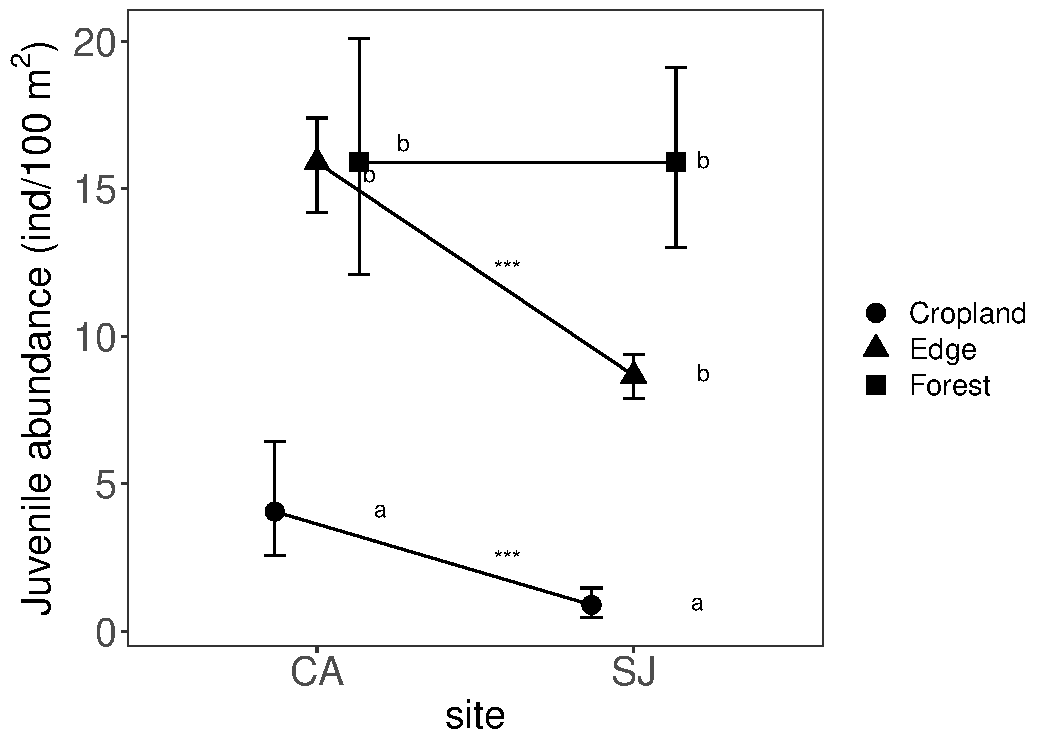
\includegraphics{/Users/ajpelu/Google Drive/_phd/03_colonization/qpyr_coloniza/ms/juvenile_interaction.pdf}

--\textgreater{} menor competencia en CA

Nagelkerke, N. J. (1991). A note on a general definition of the
coefficient of determination. Biometrika, 78(3), 691-692.

\hypertarget{refs}{}
\begin{CSLReferences}{1}{0}
\leavevmode\hypertarget{ref-CMA2007MapaUsos}{}%
CMA. 2007. \emph{Mapa de Usos y Coberturas de {Andalucía}
1956-1999-2003, 1:25 000.} {Consejería de Medio Ambiente, Junta de
Andalucía, Sevilla, Spain}.

\leavevmode\hypertarget{ref-MorenoLlorcaetal2016HistoricalAnalysis}{}%
Moreno-Llorca, R. A., A. J. P'erez-Luque, F. J. Bonet, and Zamora R.
2016. {``Historical Analysis of Socio-Ecological Changes in the
Municipality of {Cáñar} ({Alpujarra}, {Sierra Nevada}) over the Last 5
Centuries.''} In \emph{Global Change Impacts in {Sierra Nevada}:
Challenges for Conservation}, edited by R. Zamora, A. J. P'erez-Luque,
F. J. Bonet, J. M. Barea-Azc'on, and R. Aspizua, 59--62. {Consejería de
Medio Ambiente y Ordenación del Territorio. Junta de Andalucía}.

\leavevmode\hypertarget{ref-MorenoLlorcaetal2014CaracterizacionFuentes}{}%
Moreno-Llorca, Ricardo A., Antonio Jes'us P'erez-Luque, Francisco Javier
Bonet, Ram'on P'erez-P'erez, and Regino Zamora. 2014. {``Caracterización
de Fuentes de Información Para La Reconstrucción Histórica de La
Vegetación. {Un} Caso de Estudio En {Sierra Nevada}.''} In \emph{{XII
Congreso Nacional} de {Medio Ambiente} ({CONAMA} 2014)}.
\url{http://www.conama11.vsf.es/conama10/download/files/conama2014/CT}.

\leavevmode\hypertarget{ref-NavarroGonzalezetal2012CartografiaHistorica}{}%
Navarro-Gonz'alez, I., F. J. Bonet-Garc'ıa, and A. J. P'erez-Luque.
2012. {``Cartografía Histórica de La Vegetación Mediante Ortofotos.''}
In \emph{Observatorio de {Cambio Global} de {Sierra Nevada}.
{Metodologías} de Seguimiento}, edited by R. Aspizua, JM Barea-AzcNANAn,
FJ Bonet, AJ P'erez-Luque, and R. Zamor, 16--17. {Consejería de Medio
Ambiente. Junta de Andalucía}.

\leavevmode\hypertarget{ref-Piasetal2014ColonizationAbandoned}{}%
P'ıas, Beatr'ız, Gema Escribano-Avila, Emilio Virg'os, Virginia
Sanz-P'erez, Adri'an Escudero, and Fernando Valladares. 2014. {``The
Colonization of Abandoned Land by {Spanish} Juniper: {Linking} Biotic
and Abiotic Factors at Different Spatial Scales.''} \emph{Forest Ecology
and Management} 329 (October): 186--94.
\url{https://doi.org/10.1016/j.foreco.2014.06.021}.

\leavevmode\hypertarget{ref-ValbuenaCarabanaetal2010HistoricalRecent}{}%
Valbuena-Carabaña, M., U. L. de Heredia, P. Fuentes-Utrilla, I.
Gonz'alez-Doncel, and L. Gil. 2010. {``Historical and Recent Changes in
the {Spanish} Forests: A Socio-Economic Process.''} \emph{Review of
Palaeobotany and Palynology} 162 (3): 492--506.

\leavevmode\hypertarget{ref-ZamoraBareaAzcon2015LongTermChanges}{}%
Zamora, Regino, and Jos'e Miguel Barea-Azc'on. 2015. {``Long-{Term
Changes} in {Mountain Passerine Bird Communities} in the {Sierra Nevada}
({Southern Spain}): {A} 30-{Year Case Study}.''} \emph{Ardeola} 62 (1):
3--18. \url{https://doi.org/10.13157/arla.62.1.2015.3}.

\end{CSLReferences}

\end{document}
